%%%%%%%%%%%%%%%%%%%%%%%%%%%%%%%%%%%%%%%%%%%%%%%%%%%%%%%%%%%%%%%%%%%%%%%%
% Plantilla TFG/TFM
% Escuela Politécnica Superior de la Universidad de Alicante
% Realizado por: Jose Manuel Requena Plens
% Contacto: info@jmrplens.com / Telegram:@jmrplens
%%%%%%%%%%%%%%%%%%%%%%%%%%%%%%%%%%%%%%%%%%%%%%%%%%%%%%%%%%%%%%%%%%%%%%%%


% Ejemplo de páginas en horizontal y vertical

\chapter{Salidas de GTKWave de las implementaciones de \gls{cordic}}
A continuación se muestran las salidas del programa GTKWave de las distintas implementaciones: básica, \textit{pipelining} y punto flotante. Este programa es similar a otros productos comerciales, pero con la ventaja de ser de código libre. Se ha usado el programa extensivamente para encontrar errores durante el desarrollo del trabajo y ha sido de gran utilidad para entender el funcionamiento interno de cada implementación, sobre todo en la de punto flotante, donde se verá que hay una mayor cantidad de registros a tener en cuenta y manipular.

\begin{landscape} % Inicia modo horizontal
	\begin{figure}[ht]
		\centering
		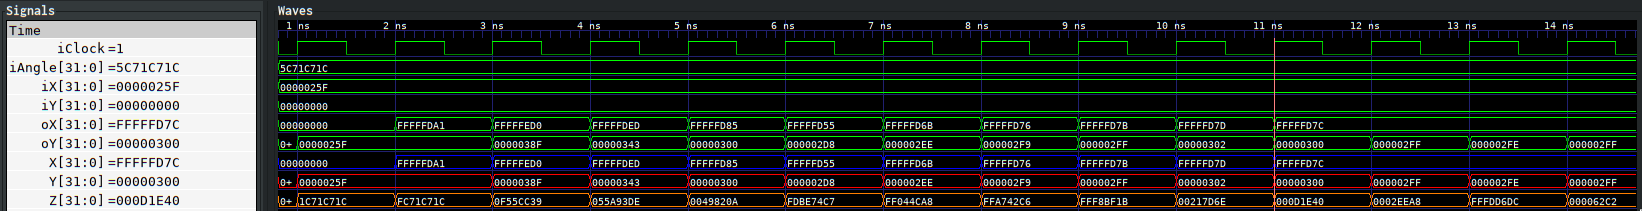
\includegraphics[width=\paperwidth]{archivos/CORDIC/salida_gtkwave_basico.png}
		\caption{Salida de GTKWave de \gls{cordic} básico}
		\label{graf:salida_gtkwave_basico}
	\end{figure}
	\clearpage

	\begin{figure}[ht]
		\centering
		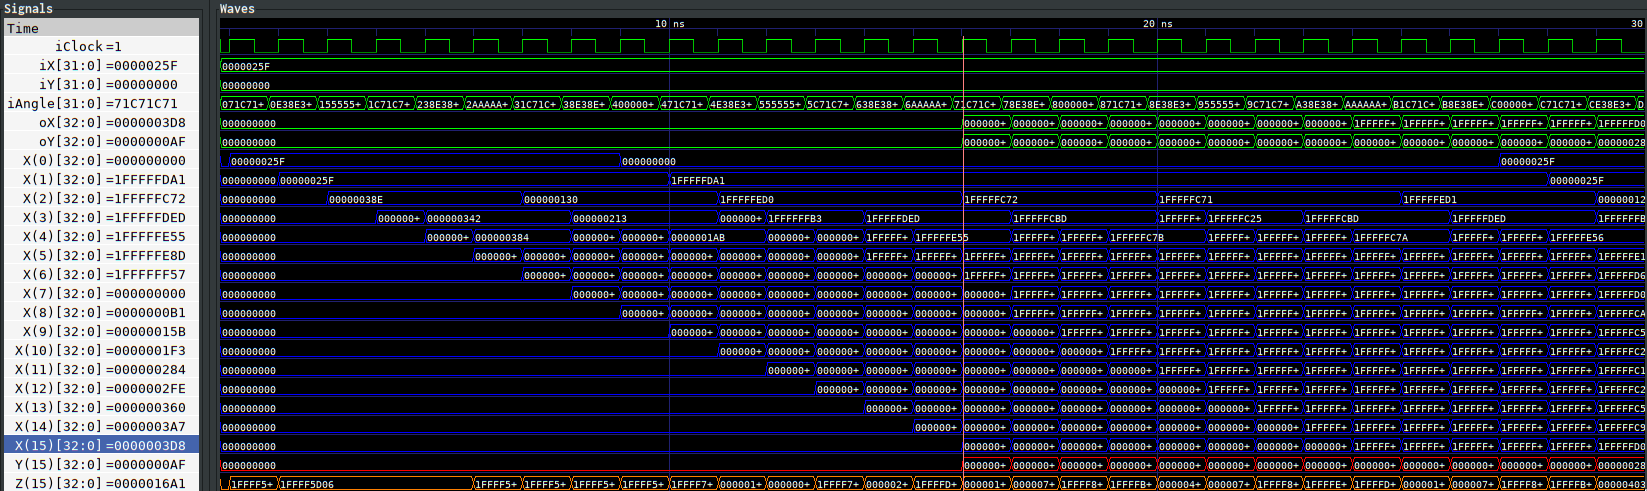
\includegraphics[width=\paperwidth]{archivos/CORDIC/salida_gtkwave_pipeline.png}
		\caption{Salida de GTKWave de \gls{cordic} con \textit{pipelining}. Aquí se muestran todos los registros de $X$ y solo los últimos registros de $Y$ y $Z$, además de las entradas y salidas.}
		\label{graf:salida_gtkwave_pipeline}
	\end{figure}
	\clearpage % Nueva página
	
	\begin{figure}[ht]
	\centering
	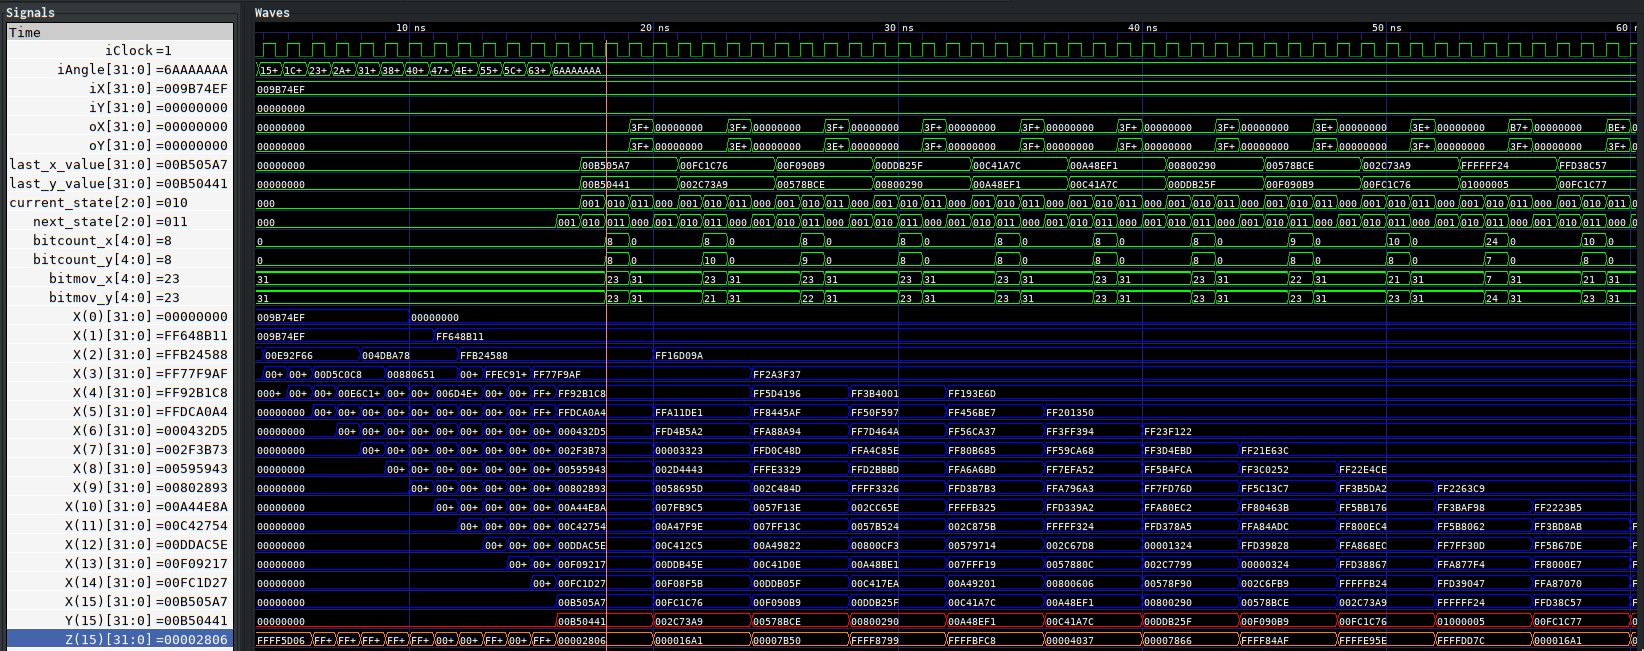
\includegraphics[width=\paperwidth]{archivos/CORDIC/salida_gtkwave_fp2.png}
	\caption{Salida de GTKWave de \gls{cordic} con punto flotante y \textit{pipelining}. Igual que en la figura anterior, se muestra todos los registros de $X$ y solo los últimos registros de $Y$ e $Z$. Además se muestran registros como \textit{next\_state} y \textit{current\_state} y otras, como contadores.}
	\label{graf:salida_gtkwave_fp}
	\end{figure}
	\clearpage
	

	
\end{landscape} % Finaliza modo horizontal

